The backend's logic is organized into several distinct modules, each responsible for a specific domain of functionality. This modular design enhances maintainability and allows for a clear separation of concerns, as depicted in the module diagram in Figure~\ref{FIG:BACKEND_MODULES}.

\begin{figure}[Backend Module Diagram]{FIG:BACKEND_MODULES}{Backend Module Diagram.}
    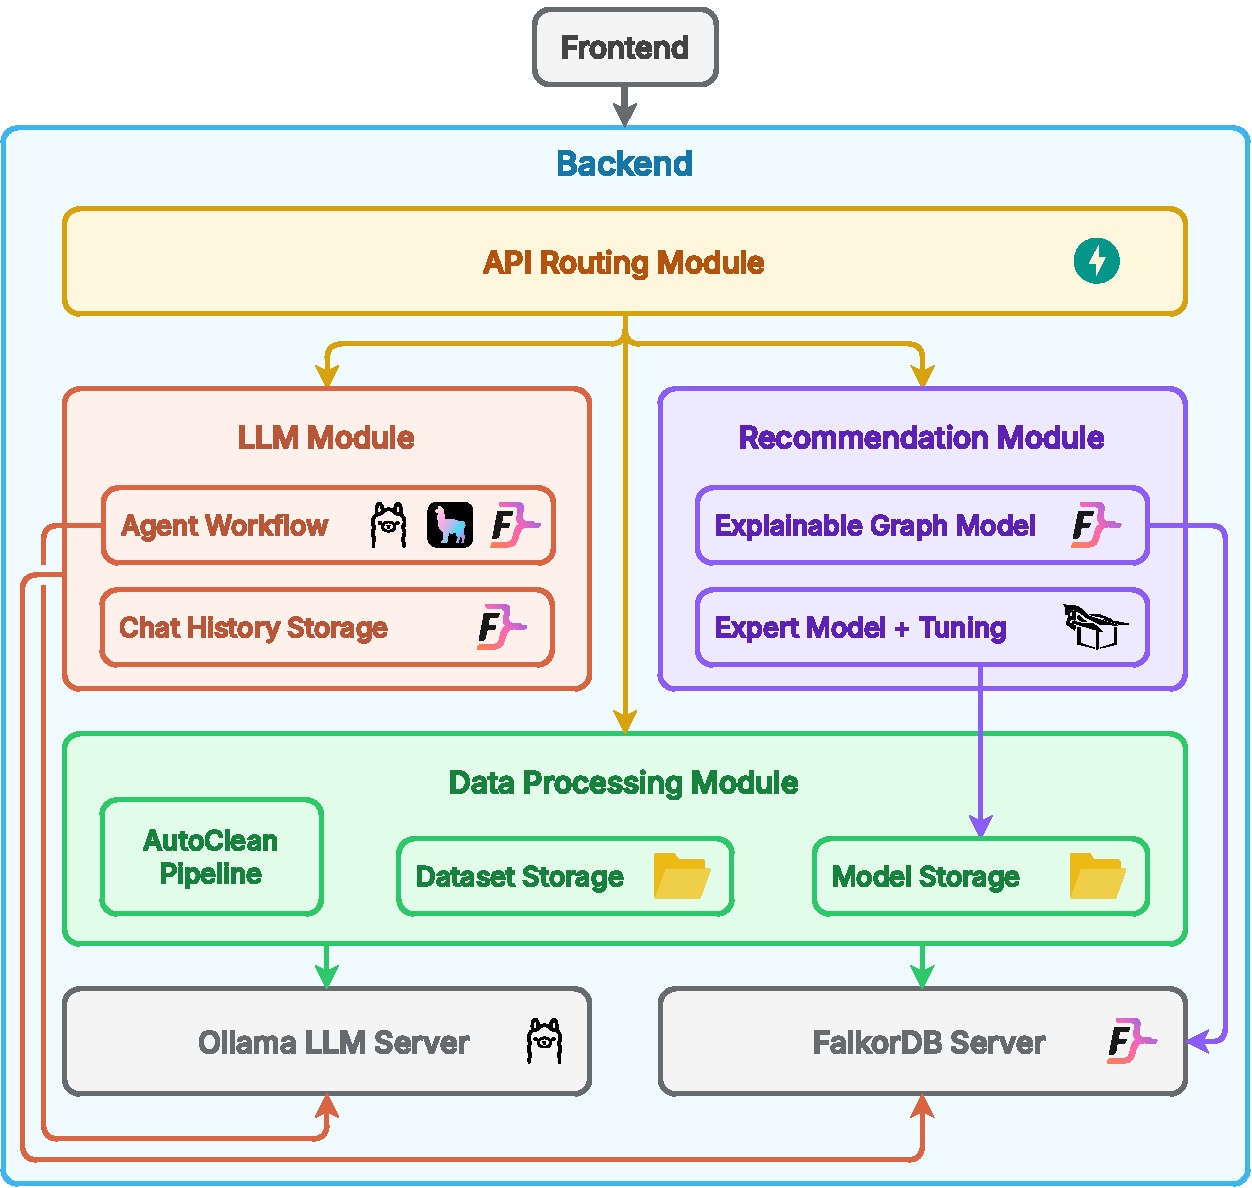
\includegraphics[width=0.9\textwidth]{backend_modules.pdf}
\end{figure}

The core modules are defined as follows:
\begin{description}
    \item[\acs{api} Routing Module] This is the main entry point of the backend, built using FastAPI. It is responsible for defining all HTTP endpoints, handling request validation through Pydantic schemas, managing user authentication through a middleware, and delegating tasks to the appropriate domain logic modules.

    \item[\acs{llm} Module] This module encapsulates all interactions with the language models and the graph database. It utilizes the LlamaIndex framework to manage the conversational agent's logic, including streaming events and Function Calling. It is also responsible for managing user profiles during a conversation and persisting chat histories to the graph database as nodes.

    \item[Recommendation Module] This module contains all logic related to generating recommendations. It is further subdivided into two major components: a graph-based recommender using FalkorDB for real-time, explainable recommendations, and an expert model from RecBole to train on the datasets---including new session interactions---and serve predictions.

    \item[Data Processing Module] This module handles the asynchronous, time-consuming tasks related to agent creation. When a user uploads new datasets, this module executes a pipeline that cleans the data, prepares it for the different recommender components, and triggers the model training and data ingestion processes.
\end{description}